\section{Mailserver aufsetzen}

\subsection{Statische IP-Adresse}
Die IP-Adresse, durch welche der Computer im Netz eindeutig identifiziert wird, sieht möglicherweise nach jedem Computerstart anders aus. Damit der Router im Heimnetzwerk später weiss, wohin er die einkommenden Mails weiterleiten muss, sollte die IP-Adresse statisch festgelegt werden.
\\
\\
Zuerst muss die Netwerkkonfigurationsdatei unter \textit{etc/network/interfaces} angepasst werden.
\\
Dazu muss man die Datei mit einem Texteditor öffnen. Dazu kann der vorinstallierte Texeditor \textit{Nano} verwendet werden:

\begin{lstlisting}
sudo nano /etc/network/interfaces
\end{lstlisting}

\begin{figure}[H]
\centering
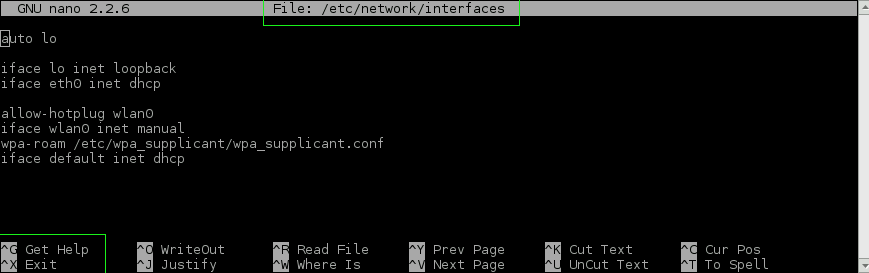
\includegraphics[scale=0.6]{images/nano}
\caption{Texteditor Nano}
\end{figure}

Unter Umständen kann es vorkommen, dass folgende Zeile bereits in der Datei steht:

\begin{lstlisting}
iface eth0 inet dhcp
\end{lstlisting}

Sofern dies der Fall ist, muss diese gelöscht und durch folgende Zeilen ersetzt werden:

\begin{lstlisting}
iface eth0 inet static
address 192.168.1.107
netmask 255.255.255.0
gateway 192.168.1.1
network 192.168.1.0
broadcast 192.168.1.255
\end{lstlisting}

Die verwendete IP-Adresse in der zweiten Zeile (192.168.1.107) sollte durch die aktuelle IP-Adresse des Systems ersetzt werden. Diese kann mit dem Kommando \textit{ifconfig} ermittelt werden. Sie steht auf der zweiten Zeile bei \textit{eth0} unter \textit{inet addr:}.

\begin{figure}[H]
\centering
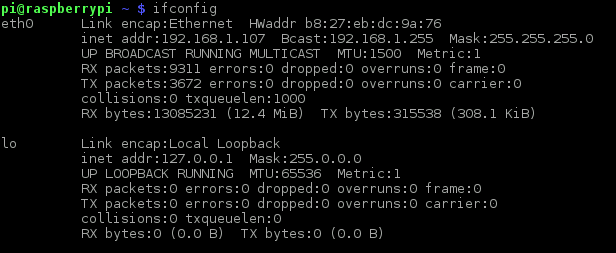
\includegraphics[scale=0.65]{images/ifconfig}
\caption{Ausgabe von ifconfig}
\end{figure}

\subsection{Voraussetzung einer Domain}
Damit ein Mailserver immer erreichbar ist, braucht es auf irgendeinem Domain Name Server einen Eintrag. Dies bedeutet, dass die Verbindung von unserem lokalen Router zu einem beliebigen anderen Computer im Internet gewährleistet ist.
... to be continued

%\section{Mailordner verschlüseln}
%Der Ordner, in dem später die Mails aufbewahrt werden, soll verschlüsselt werden (engl.: to encrypt). Dazu benutzt man das Programm EncFS.

%Zuerst muss das Kernelmodul FUSE geladen werden.

%\begin{lstlisting}
%modprobe fuse
%\end{lstlisting}

%Danach kann EncFS installiert werden mit:
%\begin{lstlisting}
%apt-get install encfs
%\end{lstlisting}

%Anschliessend kann die Konfiguration vorgenommen werden. Dazu kann man einfach folgende Befehle kopieren und in der Konsole absetzen.

%\begin{lstlisting}
%mkdir /encrypted-mail /decrypted-mail
%chgrp mail /decrypted-mail/
%chmod -R g+rw /decrypted-mail/
%gpasswd -a mail fuse
%chgrp fuse /dev/fuse; chmod g+rw /dev/fuse
%encfs /encrypted-mail /decrypted-mail -o --public
%\end{lstlisting}

%Bei der Frage nach dem Modus, muss man den Paranoia Mode auswählen. Einfach mittels Eingabe von p bestätigen. Danach verlangt das Programm noch das Setzen eines Passwortes. Einmal gesetzt, sollte es gut aufbewahrt werden!

\subsection{Komponenten installieren}
Als nächstes müssen alle benötigten Komponenten installiert werden.
Diese sind:
\begin{itemize}
\item MySQL Server \\
MySQL bezeichnet eine Datenbank. Das zu installierende Paket stellt eine Datenbank für die E-Mail-Benutzer und andere Einstellungen zur Verfügung.

% FIXME: Description
\item Postfix \\
% FIXME: Description

\item Dovecot \\
% FIXME: Description

\end{itemize}

Dovecot verlangt ein aktives IPv6-Modul. Dieses muss zur entsprechenden Liste hinzugefügt und anschliessend aktiviert werden:

\begin{lstlisting}
echo "ipv6" >> /etc/modules
modprobe ipv6
\end{lstlisting}

Nun können die Pakete installiert werden:

\begin{lstlisting}
apt-get install postfix postfix-mysql dovecot-common dovecot-imapd mysql-server dovecot-pop3d openssl
\end{lstlisting}

Nachfolgend werden der Reihe nach für MySQL und Postfix gewisse Grundeinstellunen vorgenommen. Die Programme führen den Benutzer dabei an der Hand und gehen Schritt für Schritt die Fragen durch.

% FIXME: Screenshots einfügen + Text (caption?)

Anschliessend werden alle Pakete installiert, was ein paar Minuten dauern kann.

\subsubsection{MySQL}
Zuerst muss die MySQL-Datenbank mit dem Namen "postfix" erstellt werden. Dies geschieht mit dem folgenden Befehl:

\begin{lstlisting}
mysqladmin -p create postfix
\end{lstlisting}

Nun wird man nach dem Passwort gefragt. Es handelt sich dabei um jenes, welches während der Installation von MySQL gewählt wurde.

Anschliessend kann man sich in die Datenbank einloggen. Es wird erneut nach dem gleichen Passwort gefragt:

\begin{lstlisting}
mysql -p postfix
\end{lstlisting}

Ein Benutzer für die Datenbank postfix wird jetzt angelegt:

\begin{lstlisting}
CREATE USER 'postfix'@'localhost' IDENTIFIED BY 'SOMEPASSWORD';
GRANT ALL PRIVILEGES ON postfix.* TO 'postfix'@'localhost' IDENTIFIED BY 'SOMEPASSWORD';
FLUSH PRIVILEGES;
\end{lstlisting}

\subsection{Postfix Administrationstool}

Damit wir keine manuellen Anpassungen an der Datenbank vornehmen müssen, wie z.B. Tabellen, Benutzer, E-Mail-Adressen und so weiter erstellen, installieren wir uns \textit{Postfix admin} ein Administrationstool um Postfix zu konfigurieren. \\

Dieses Tool ist leider nicht über unsere Paketverwaltung verfügbar, weshalb wir es aus dem Internet herunterladen und selbst in unser Webserververzeichnis \textit{/var/www} verschieben müssen:

\begin{lstlisting}
cd /var/www
wget --content-disposition http://sourceforge.net/projects/postfixadmin/files/latest/download?source=files
tar xfvz postfixadmin-*.tar.gz
mv postfixadmin*/ postfixadmin
chown www-data:www-data -R postfixadmin
cd postfixadmin
\end{lstlisting}

Damit \textit{postfix admin} eine Verbindung zu unserer Datenbank herstellen kann, müssen wir einige Anpassungen vornehmen. Folgende Werte müssen in der Datei \textit{/var/www/postfixadmin/config.inc.php} gesucht und entsprechend angepasst werden:

\begin{lstlisting}
$CONF['configured'] = true;
$CONF['database_type'] = 'mysql';
$CONF['database_host'] = 'localhost';
$CONF['database_user'] = 'postfix';
$CONF['database_password'] = 'SOMEPASSWORD';
$CONF['database_name'] = 'postfix';
$CONF['encrypt'] = 'md5crypt';
$CONF['domain_path'] = 'YES';
$CONF['default_language'] = 'de';
$CONF['domain_in_mailbox'] = 'NO';
$CONF['emailcheck_resolve_domain'] = 'NO';
\end{lstlisting}

In der selben Datei kommt oft die Beispielsdomain \textit{change-this-to-your.domain.tld} vor. Diese muss durch die Domain ersetzt werden, die man bei der Installation von \textit{postfix} angegeen hat.

Nun kann mit dem Setup von \textit{postfix} begonnen werden. Dazu einfach in einem Webbroser eure Domain wie folgt aufrufen:

\begin{lstlisting}
http://deinedomain.tld/postfixadmin/setup.php
\end{lstlisting}

Hierbei wird ein Check ausgeführt, wo alle Abhängigkeiten geprüft werden. Steht da überall \textit{OK} kann weitergefahren werden, ansonsten müssen die Abhängigkeiten installiert oder Konfigurationen angepasst werden. \\
Zusätzlich wird nach einem \textit{setup password} gefragt. Dieses sollte auf jeden Fall gesetzt werden und wird dazu gebraucht um sich bei einem weiteren Setupaufruf identifizieren zu können.
Dieses Setuppassword muss anschliessend auch in die Datei \textit{/var/www/postfixadmin/config.inc.php} eingetragen werden.

\begin{lstlisting}
$CONF['setup_password'] = 'GEWAEHLTESSETUPPASSWORT';
\end{lstlisting}

Nun muss erneut die Setup Seite aufgerufen und ein Administrationkonto angelegt werden. Dieses wird gebraucht, um später E-Mail-Adressen und weiteres anzulegen.

\subsubsection{Postfix}
Da wir nun \textit{postfix admin} installiert und konfiguriert haben, können wir mit der eigentlichen \textit{postfix} Konfiguration beginnen.

Damit nur ein bestimmter Benutzer unseres System für den Mailserver Teil verantwortlich ist, legen wir diesen an. Wir folgenen gewissen Linux-Richtlinien und geben diesem E-Mail Benutzer die ID \textit{5000}:

\begin{lstlisting}
mkdir /var/vmail
groupadd -g 5000 vmail
useradd -g vmail -u 5000 vmail -d /var/vmail
chown vmail:vmail /var/vmail
\end{lstlisting}

Sicherheitstechnisch ist es zudem sehr wichtig, dass \textit{postfix} eine SSL-Verbindung hat. Dazu erstellen wir ein Zertifikat mit \textit{openssl}

\begin{lstlisting}
mkdir /etc/postfix/sslcert
cd /etc/postfix/sslcert
openssl req -new -newkey rsa:3072 -nodes -keyout postfix.key -days 730 -x509 -out postfix.crt
chmod go-rwx postfix.key
\end{lstlisting}

Beim Erstellen des Zertifikates werden einige Informationen benötigt. Vorallem ist hier wichtig, dass bei dem \textit{Command Name}-Frage die Domain angegeben wird, mit dem auch \textit{postfix} konfiguriert wurde.

Weiter geht es mit der Hauptkonfiguration von \textit{postfix}. \\
Wir fügen der Datei \textit{/etc/postfix/main.cf} folgendes hinzu:

\begin{lstlisting}
disable_vrfy_command = yes
smtpd_sasl_type=dovecot
smtpd_sasl_path=private/auth_dovecot
smtpd_sasl_auth_enable = yes
smtpd_sasl_authenticated_header = yes
broken_sasl_auth_clients = yes
proxy_read_maps = $local_recipient_maps $mydestination $virtual_alias_maps $virtual_alias_domains $virtual_mailbox_maps $virtual_mailbox_domains $relay_recipient_maps $relay_domains $canonical_maps $sender_canonical_maps $recipient_canonical_maps $relocated_maps $transport_maps $mynetworks $smtpd_sender_login_maps
smtpd_sender_login_maps = proxy:mysql:/etc/postfix/mysql_sender_login_maps.cf
smtpd_sender_restrictions = reject_authenticated_sender_login_mismatch
                reject_unknown_sender_domain
smtpd_recipient_restrictions = permit_sasl_authenticated
                permit_mynetworks
                reject_unauth_destination

# Virtual mailboxes
local_transport = virtual
virtual_alias_maps = proxy:mysql:/etc/postfix/mysql_virtual_alias_maps.cf
virtual_mailbox_base = /var/vmail/
virtual_mailbox_domains = proxy:mysql:/etc/postfix/mysql_virtual_domains_maps.cf
virtual_mailbox_limit = 524288000
virtual_mailbox_maps = proxy:mysql:/etc/postfix/mysql_virtual_mailbox_maps.cf
virtual_minimum_uid = 104
virtual_transport = virtual
virtual_uid_maps = static:5000
virtual_gid_maps = static:5000
virtual_transport = dovecot
dovecot_destination_recipient_limit = 1
\end{lstlisting}

In dieser Datei ist auch wichtig, dass der Eintrag \textit{mydestination} nur \textit{localhost} enthält:

\begin{lstlisting}
mydestination = localhost
\end{lstlisting}

Zudem muss man auf die vorher erstellen SSL-Zertifikate verweisen:

\begin{lstlisting}
smtpd_tls_cert_file = /etc/postfix/sslcert/postfix.crt
smtpd_tls_key_file = /etc/postfix/sslcert/postfix.key
\end{lstlisting}

Eine weitere wichtige Konfigurationsdatei von \textit{postfix} ist \textit{/etc/postfix/master.cf}. \\
Folgendes muss dieser Datei hinzugefügt werden:

\begin{lstlisting}
dovecot   unix  -       n       n       -       -       pipe
  flags=DRhu user=vmail:vmail argv=/usr/lib/dovecot/deliver -d ${recipient}
\end{lstlisting}

\textbf{Wichtig:} Die Einrückung der zweiten Zeile muss unbedingt eingehalten werden. Dies gilt auch für weitere Anpassungen in dieser Datei.

Für die folgenden beiden Zeilen muss die Raute (\#) davor entfernt werden, um sie aktiv zu machen:

\begin{lstlisting}
submission inet n       -       -       -       -       smtpd
  -o smtpd_tls_security_level=encrypt
  -o smtpd_client_restrictions=permit_sasl_authenticated,reject
smtps     inet  n       -       -       -       -       smtpd
  -o smtpd_tls_wrappermode=yes
\end{lstlisting}


Nicht nur \textit{postfix admin} braucht eine Verbindung zu unseren Datenbank, auch \textit{postfix} selbst braucht eine. Dazu folgende Dateien mit entsprechendem Inhalt erstellen:

\begin{lstlisting}
nano /etc/postfix/mysql_virtual_alias_maps.cf
\end{lstlisting}

\begin{lstlisting}
hosts = localhost
user = postfix
password = SOMEPASSWORD
dbname = postfix
query = SELECT goto FROM alias WHERE address='%s' AND active = '1'
\end{lstlisting}

\begin{lstlisting}
nano /etc/postfix/mysql_virtual_mailbox_maps.cf
\end{lstlisting}

\begin{lstlisting}
hosts = localhost
user = postfix
password = SOMEPASSWORD
dbname = postfix
query = SELECT maildir FROM mailbox WHERE username='%s' AND active = '1'
\end{lstlisting}

\begin{lstlisting}
nano  \etc/postfix/mysql_virtual_domains_maps.cf
\end{lstlisting}

\begin{lstlisting}
hosts = localhost
user = postfix
password = SOMEPASSWORD
dbname = postfix
query = SELECT domain FROM domain WHERE domain='%s' AND active = '1'
\end{lstlisting}

\begin{lstlisting}
nano  \etc/postfix/mysql_sender_login_maps.cf
\end{lstlisting}

\begin{lstlisting}
hosts = localhost
user = postfix
password = SOMEPASSWORD
dbname = postfix
query = SELECT username AS allowedUser FROM mailbox WHERE username="%s" AND active = 1 UNION SELECT goto FROM alias WHERE address="%s" AND active = 1
\end{lstlisting}

Damit diese Dateien geschützt sind, sollte man die Zugriffsrechte ändern:

\begin{lstlisting}
chmod o-rwx,g+r /etc/postfix/mysql_*
chgrp postfix /etc/postfix/mysql_*
\end{lstlisting}

Postfix muss nun neu gestartet werden, damit die vorgenommenen Änderungen übernommen werden:

\begin{lstlisting}
service postfix restart
\end{lstlisting}

\subsubsection{Dovecot}
Nachdem die Konfiguration von Postfix abgeschlossen ist, kann \textit{dovecot} konfiguriert werden. \\
Als erstes ist es wichtig eine Sicherheitskopie der Originalkonfiguration zu machen, sodass im Fall einer kompletten Verwüstung dieser Abhilfe geschafft werden kann:

\begin{lstlisting}
mv /etc/dovecot/dovecot.conf /etc/dovecot/dovecot.conf.orig
\end{lstlisting}

Nun kann eine komplett neue Konfigurationsdatei angelegt werden und mit folgendem Inhalt befüllt werden:

\begin{lstlisting}
nano /etc/dovecot/dovecot.conf
\end{lstlisting}

\begin{lstlisting}
auth_mechanisms = plain login
log_timestamp = "%Y-%m-%d %H:%M:%S "
passdb {
  args = /etc/dovecot/dovecot-mysql.conf
  driver = sql
}
protocols = imap pop3
service auth {
  unix_listener /var/spool/postfix/private/auth_dovecot {
    group = postfix
    mode = 0660
    user = postfix
  }
  unix_listener auth-master {
    mode = 0600
    user = vmail
  }
  user = root
}
listen = *
ssl_cert = </etc/postfix/sslcert/postfix.crt
ssl_key = </etc/postfix/sslcert/postfix.key
userdb {
  args = /etc/dovecot/dovecot_mysql.conf
  driver = sql
}
protocol pop3 {
  pop3_uidl_format = %08Xu%08Xv

}
protocol lda {
  auth_socket_path = /var/run/dovecot/auth-master
  postmaster_address = postmaster@unseredomain.tld
}
\end{lstlisting}

In dieser Datei gibt man in der \textit{userdb} Konfiguration eine Datei für die SQL-Verbindung an. Diese muss natürlich nun erstellt und mit folgendem Inhalt befüllt werden:

\begin{lstlisting}
driver = mysql
connect = host=localhost dbname=postfix user=postfix password=SOMEPASSWORD
default_pass_scheme = MD5-CRYPT
password_query = SELECT password FROM mailbox WHERE username = '%u'
user_query = SELECT CONCAT('maildir:/var/vmail/',maildir) AS mail, 5000 AS uid, 5000 AS gid FROM mailbox WHERE username = '%u'
\end{lstlisting}

Auch diese Datei sollte wieder mit Zugriffsrechten versehen werden, die es nicht erlauben, dass die Datei von jedem Benutzer gelesen werden kann:

\begin{lstlisting}
chmod o-rwx,g+r /etc/dovecot/dovecot_mysql.conf
chgrp vmail /etc/dovecot/dovecot_mysql.conf
\end{lstlisting}

Damit die Änderungen korrekt übernommen werden können, starten wir \textit{dovecot} neu:

\begin{lstlisting}
service dovecot restart
\end{lstlisting}

\subsection{Erste E-Mail Adresse anlegen}
Nachdem die Konfiguration von \textit{postfix} und \textit{dovecot} abgeschlossen ist, kann man mit der Erfassung von E-Mail Adressen beginnen. Nicht umsonst haben wir \textit{postfix admin} installiert. Dies kommt nun zum Einsatz. Surft man auf die Seite \textit{http://unseredomain.tld/postfixadmin} kann man sich dort mit dem Administrationsbenutzer einloggen und mit der Erfassung beginnen.

Bevor man eine E-Mail Adresse erfassen kann, muss man eine Domain konfigurieren. Diese Domain ist jene, auf der wir uns gerade befinden. \\
Dazu geht man in \textit{postfix admin} auf:

\begin{lstlisting}
Domain Liste -> Neue Domain
\end{lstlisting}

Und legt jene dort an:

\begin{figure}[H]
\centering
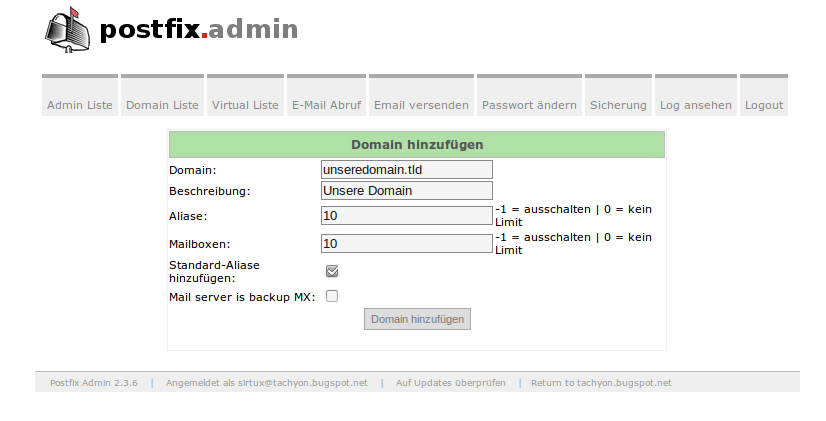
\includegraphics[scale=0.3]{images/pa-domain.png}
\caption{Postfix admin - Neue Domain}
\end{figure}

Als nächstes kann die E-Mail Adresse eingerichtet werden. Dazu geht man auf:

\begin{lstlisting}
Virtual Liste -> Mailbox hinzufuegen
\end{lstlisting}

\begin{figure}[H]
\centering
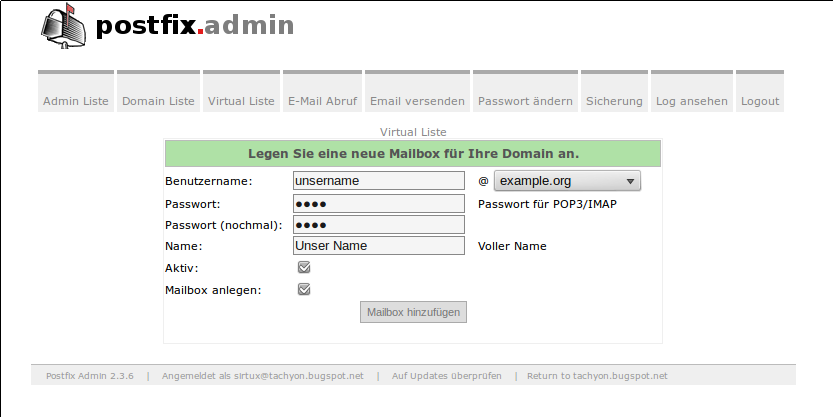
\includegraphics[scale=0.3]{images/pa-mail.png}
\caption{Postfix admin - Neue Mailbox}
\end{figure}
